\documentclass{IEEEtran}

\usepackage{graphicx}
\usepackage{hyperref}

\title{Two-Layer Hidden Markov Models Based Music Emotion Classification}
\author{Sihan Li\\2013011187\\lisihan969@gmail.com}

\begin{document}
  \maketitle

  \begin{abstract}
    Music classification has received much attention in the last decades.
    Emotion is one of the criteria used for classification. Its applications
    include automatic music recommendation, background music selection and
    so on. In this paper, we proposed a two-layer Hidden Markov Models (HMM)
    based music emotion classification methodology. Four Layer-1 HMMs
    classify 25~ms music clips while one layer-2 HMM judges emotion from 10~s music clips.
    In this way the emotion is determined by both short-term information
    (tones) and long-term information (melodies). The experiments show that
    our model.

  \end{abstract}

  \section{Introduction}

  Music has become a part of our daily life. Many products and services have been
  produced to give people best music experience. Among these services,
  automatic music recommendation has received much attention, as it gives users
  the ability to discover new musics that are likely to be in users' favor.
  In such an application, simply classification based on traditional genres
  (pop, fork, classic, etc.) is usually not enough, as songs that share a genre may
  convey different emotions. As a result, music emotion classification has
  received much attention. Yang proposed fuzzy approach to the problem. They
  implemented two fuzzy classifiers to measure the strength of the emotion.
  \cite{yang2006music}. Multi-modal classification which takes lyrics into
  consideration was studied in a following research \cite{yang2008toward}.

  On the other side, more research has been conducted in general music
  classification. West conducted a comprehensive research on music
  classification in \cite{west2008novel}. Features extraction, as well as
  classification algorithms have been discussed in the paper. Hidden Markov
  Models (HMM) based classification was first proposed by Chai
  \cite{chai2001folk}. They applied different HMM to symbolic folk musics to
  perform a 2-way or 3-way classification. Later Karpov did a more thorough
  research using HMM on digital musics \cite{karpov2002hidden}. Features
  including MFCC are extracted from the musics first. They are then treated
  as the emissions of the HMM. Their works, with Durey's survey
  \cite{durey2001melody}, prove that HMM, which was mostly used in speech
  recognition before \cite{rabiner1989tutorial}, could be applied to music
  classification with a satisfactory result.

  However, none of the above research has discussed about the application of
  HMM in music emotion classification. Moreover, considering that emotion is
  continuously changed in a song, it also has long-term Markov
  properties, which is discarded by all the works listed above as they cut
  the music into small clips first. Thus, in this paper, we proposed a
  two-layer Hidden Markov Models based music emotion classification method. We
  first implemented four layer-1 HMMs to classify 10-second music clips. They
  take 25~ms music clips as input, and output the probabilities for each
  emotion category. A layer-2 HMM is then used to judge the emotion from the
  probability vectors. In this way we can utilize both local and global emotion
  information.

  The rest of the paper is organized as follows. Section~\ref{sec:Model}
  describes the detail of the proposed model. Section~\ref{sec:Implementation}
  shows the way we implemented our model. Section~\ref{sec:Result} gives the
  result of our experiments. Section~\ref{sec:Conclusion} draw a conclusion,
  and Section~\ref{sec:Discussion} discusses the possible following research.

  \section{Model}
  \label{sec:Model}

  To classify a music according to the emotions it contains, one has to first
  define emotions. Thayer proposed a model which classifies emotions
  according to two criteria: valence and arousal
  \cite{thayer1989biopsychology}. In this way, emotions are classifies into
  four categories, as depicted in Figure~\ref{fig:emotion}. This model was adopted by
  Yang's works \cite{yang2006music,yang2008toward}. This notation reserves
  part of the relationships between different emotions. We will use Thayer's
  emotion plane in our model.

  \begin{figure}[htbp]
    \centering
    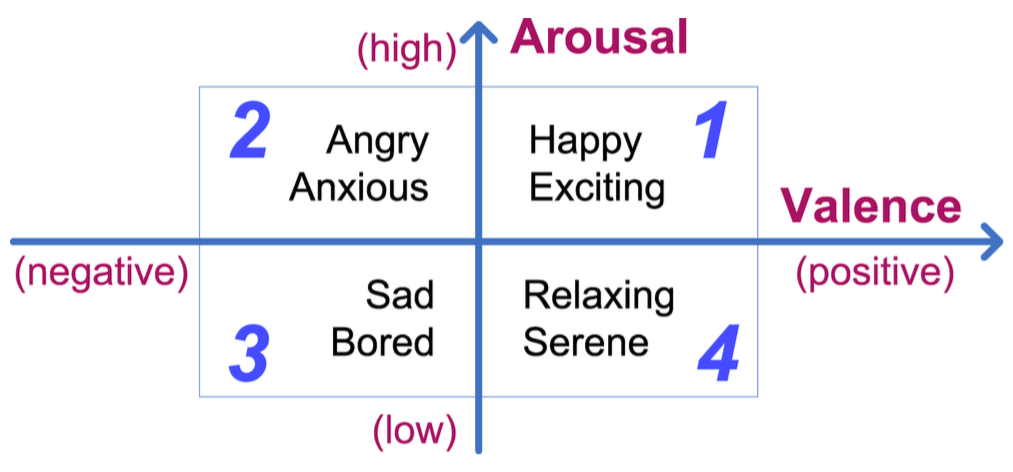
\includegraphics[width=\columnwidth]{emotion.png}
    \caption{Thayer's emotion plane. The image is taken from \cite{yang2006music}.}
    \label{fig:emotion}
  \end{figure}

  In order to utilize both short-term and long-term information, we design a
  two-layer structure. Layer-1 contains four HMMs, corresponding to four types
  of emotions. Each HMM is trained using the music clips (10~s) of the
  corresponding type, and output the probability that the clip belongs to that
  type. The probabilities are then taken to the layer-2 HMM, which is trained
  by complete songs. After given the information of the whole song, the
  layer-2 HMM will make the final decision and judge each clip's emotion type.
  The structure of our model is depicted in Figure~\ref{fig:structure}.

  \begin{figure}[htbp]
    \centering
    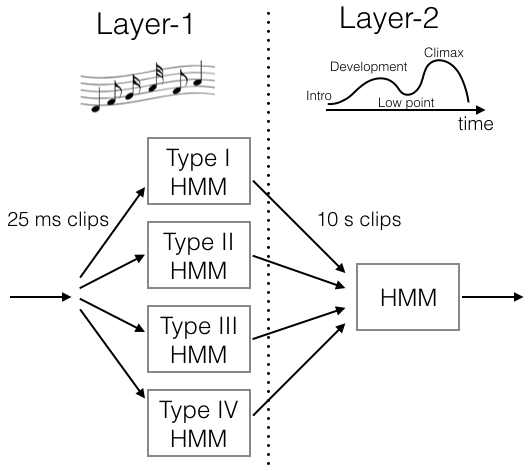
\includegraphics[width=\columnwidth]{structure.png}
    \caption{Structure of our model. Layer-1 works on short-term (25ms)Features while layer-2 works on long-term (10s) features.}
    \label{fig:structure}
  \end{figure}

  For layer-1 HMMs, 25ms MFCCs are used as emissions. For layer-2 HMM, the
  10s probabilities vectors (4-dimension) are used as emissions. Each layer-1
  HMM and layer-2 HMM has four hidden states. In layer-1, the meaning of the
  states is not clear while in layer-2, each state represents a type of
  emotion.

  \section{Implementation}
  \label{sec:Implementation}

  \subsection{Music selection}

  We first select 44 songs from soundtracks of two animes and a movie. The
  song list is carefully selected so that each song has exactly one emotion.
  These songs are used to train layer-1 HMMs. Then 15 songs from the same
  albums have been selected to train layer-2 HMMs. These songs have more
  complex structures, each song contains more than one emotions.

  \subsection{Pre-processing}
  Before processing, each song is converted into 44100Hz, mono channel format.

  For the layer-1 train set, songs are divided into no-overlapping 10 second
  clips, while for the layer-2 train set, clips are 50\%-overlapping. This is
  because each song in layer-1 train set has only one emotion, so the
  overlapping will not utilize more information. On the other hand,
  songs in layer-2 train set have long-term information. So overlapping is
  needed or some information will be missing if the an emotion transaction
  happens on the edge of a clip. The division of the train sets is shown in
  Figure~\ref{fig:trainset_division}.

  \begin{figure}[htbp]
    \centering
    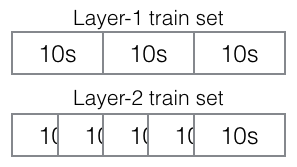
\includegraphics[width=0.6\columnwidth]{trainset_division.png}
    \caption{Trainset division for layer-1 and layer-2.}
    \label{fig:trainset_division}
  \end{figure}

  The song clips are then manually (well, by myself) classified. Each
  ten-second-clip is labeled with an emotion type (1 to 4).

  \subsection{Feature extraction}
  12 Mel frequency cepstral coefficients are taken from 25~ms clips every
  10~ms. Wojcicki's implementation is used for MFCCs extraction \cite{wojcicki2011htk}.

  \subsection{HMM setup}

  MATLAB offers a HMM implementation, but it can only handle discrete
  emissions, which is not our case. Thus we use Murphy's Hidden markov model
  toolbox for MATLAB for HMMs training \cite{murphy1998hidden}. Gaussian
  outputs models are used in our implementation.

  For layer-1 HMMs, hidden state number is chosen to four according to
  \cite{chai2001folk}.

  The source code of our implementation is available at
  \url{https://github.com/ThomasLee969/music-classification}.


  \section{Result}
  \label{sec:Result}

  \begin{figure}[htbp]
    \centering
    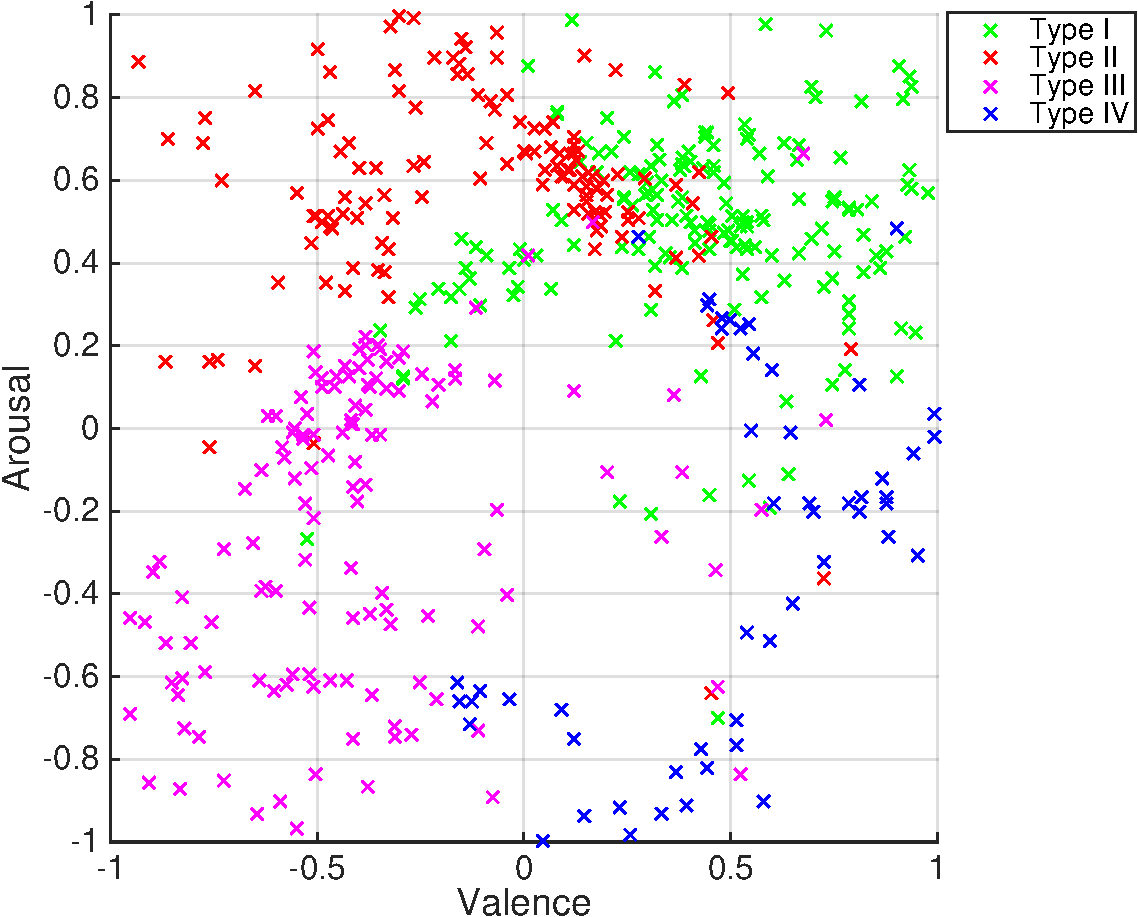
\includegraphics[width=\columnwidth]{trainset.pdf}
    \caption{Layer-1's output for layer-1 train set after training.}
    \label{fig:trainset}
  \end{figure}


  \section{Conclusion}
  \label{sec:Conclusion}

  \section{Discussion}
  \label{sec:Discussion}


  \bibliographystyle{IEEEtran}
  \bibliography{refs}

\end{document}
